\documentclass[twoside]{book}

% Packages required by doxygen
\usepackage{fixltx2e}
\usepackage{calc}
\usepackage{doxygen}
\usepackage[export]{adjustbox} % also loads graphicx
\usepackage{graphicx}
\usepackage[utf8]{inputenc}
\usepackage{makeidx}
\usepackage{multicol}
\usepackage{multirow}
\PassOptionsToPackage{warn}{textcomp}
\usepackage{textcomp}
\usepackage[nointegrals]{wasysym}
\usepackage[table]{xcolor}

% Font selection
\usepackage[T1]{fontenc}
\usepackage[scaled=.90]{helvet}
\usepackage{courier}
\usepackage{amssymb}
\usepackage{sectsty}
\renewcommand{\familydefault}{\sfdefault}
\allsectionsfont{%
  \fontseries{bc}\selectfont%
  \color{darkgray}%
}
\renewcommand{\DoxyLabelFont}{%
  \fontseries{bc}\selectfont%
  \color{darkgray}%
}
\newcommand{\+}{\discretionary{\mbox{\scriptsize$\hookleftarrow$}}{}{}}

% Page & text layout
\usepackage{geometry}
\geometry{%
  a4paper,%
  top=2.5cm,%
  bottom=2.5cm,%
  left=2.5cm,%
  right=2.5cm%
}
\tolerance=750
\hfuzz=15pt
\hbadness=750
\setlength{\emergencystretch}{15pt}
\setlength{\parindent}{0cm}
\setlength{\parskip}{3ex plus 2ex minus 2ex}
\makeatletter
\renewcommand{\paragraph}{%
  \@startsection{paragraph}{4}{0ex}{-1.0ex}{1.0ex}{%
    \normalfont\normalsize\bfseries\SS@parafont%
  }%
}
\renewcommand{\subparagraph}{%
  \@startsection{subparagraph}{5}{0ex}{-1.0ex}{1.0ex}{%
    \normalfont\normalsize\bfseries\SS@subparafont%
  }%
}
\makeatother

% Headers & footers
\usepackage{fancyhdr}
\pagestyle{fancyplain}
\fancyhead[LE]{\fancyplain{}{\bfseries\thepage}}
\fancyhead[CE]{\fancyplain{}{}}
\fancyhead[RE]{\fancyplain{}{\bfseries\leftmark}}
\fancyhead[LO]{\fancyplain{}{\bfseries\rightmark}}
\fancyhead[CO]{\fancyplain{}{}}
\fancyhead[RO]{\fancyplain{}{\bfseries\thepage}}
\fancyfoot[LE]{\fancyplain{}{}}
\fancyfoot[CE]{\fancyplain{}{}}
\fancyfoot[RE]{\fancyplain{}{\bfseries\scriptsize Generated by Doxygen }}
\fancyfoot[LO]{\fancyplain{}{\bfseries\scriptsize Generated by Doxygen }}
\fancyfoot[CO]{\fancyplain{}{}}
\fancyfoot[RO]{\fancyplain{}{}}
\renewcommand{\footrulewidth}{0.4pt}
\renewcommand{\chaptermark}[1]{%
  \markboth{#1}{}%
}
\renewcommand{\sectionmark}[1]{%
  \markright{\thesection\ #1}%
}

% Indices & bibliography
\usepackage{natbib}
\usepackage[titles]{tocloft}
\setcounter{tocdepth}{3}
\setcounter{secnumdepth}{5}
\makeindex

% Hyperlinks (required, but should be loaded last)
\usepackage{ifpdf}
\ifpdf
  \usepackage[pdftex,pagebackref=true]{hyperref}
\else
  \usepackage[ps2pdf,pagebackref=true]{hyperref}
\fi
\hypersetup{%
  colorlinks=true,%
  linkcolor=blue,%
  citecolor=blue,%
  unicode%
}

% Custom commands
\newcommand{\clearemptydoublepage}{%
  \newpage{\pagestyle{empty}\cleardoublepage}%
}

\usepackage{caption}
\captionsetup{labelsep=space,justification=centering,font={bf},singlelinecheck=off,skip=4pt,position=top}

%===== C O N T E N T S =====

\begin{document}

% Titlepage & ToC
\hypersetup{pageanchor=false,
             bookmarksnumbered=true,
             pdfencoding=unicode
            }
\pagenumbering{roman}
\begin{titlepage}
\vspace*{7cm}
\begin{center}%
{\Large Pathfinding }\\
\vspace*{1cm}
{\large Generated by Doxygen 1.8.11}\\
\end{center}
\end{titlepage}
\clearemptydoublepage
\tableofcontents
\clearemptydoublepage
\pagenumbering{arabic}
\hypersetup{pageanchor=true}

%--- Begin generated contents ---
\chapter{Hierarchical Index}
\section{Class Hierarchy}
This inheritance list is sorted roughly, but not completely, alphabetically\+:\begin{DoxyCompactList}
\item \contentsline{section}{A\+Star\+Search$<$ T $>$}{\pageref{class_a_star_search}}{}
\item \contentsline{section}{std\+:\+:hash$<$ Coordinate $>$}{\pageref{structstd_1_1hash_3_01_coordinate_01_4}}{}
\item \contentsline{section}{std\+:\+:hash$<$ Int\+Coord $>$}{\pageref{structstd_1_1hash_3_01_int_coord_01_4}}{}
\item \contentsline{section}{std\+:\+:hash$<$ Path\+Finder\+:\+:Coord\+Node $>$}{\pageref{structstd_1_1hash_3_01_path_finder_1_1_coord_node_01_4}}{}
\item \contentsline{section}{Int\+Coord}{\pageref{struct_int_coord}}{}
\item \contentsline{section}{Map}{\pageref{class_map}}{}
\item \contentsline{section}{Node$<$ T $>$}{\pageref{class_node}}{}
\item \contentsline{section}{Node$<$ Coord\+Node $>$}{\pageref{class_node}}{}
\begin{DoxyCompactList}
\item \contentsline{section}{Path\+Finder\+:\+:Coord\+Node}{\pageref{class_path_finder_1_1_coord_node}}{}
\item \contentsline{section}{Path\+Finder\+:\+:Coord\+Node}{\pageref{class_path_finder_1_1_coord_node}}{}
\end{DoxyCompactList}
\item \contentsline{section}{Path\+Finder}{\pageref{class_path_finder}}{}
\end{DoxyCompactList}

\chapter{Class Index}
\section{Class List}
Here are the classes, structs, unions and interfaces with brief descriptions\+:\begin{DoxyCompactList}
\item\contentsline{section}{\hyperlink{class_a_star_search}{A\+Star\+Search$<$ T $>$} }{\pageref{class_a_star_search}}{}
\item\contentsline{section}{\hyperlink{class_path_finder_1_1_coord_node}{Path\+Finder\+::\+Coord\+Node} }{\pageref{class_path_finder_1_1_coord_node}}{}
\item\contentsline{section}{\hyperlink{structstd_1_1hash_3_01_coordinate_01_4}{std\+::hash$<$ Coordinate $>$} }{\pageref{structstd_1_1hash_3_01_coordinate_01_4}}{}
\item\contentsline{section}{\hyperlink{structstd_1_1hash_3_01_int_coord_01_4}{std\+::hash$<$ Int\+Coord $>$} }{\pageref{structstd_1_1hash_3_01_int_coord_01_4}}{}
\item\contentsline{section}{\hyperlink{structstd_1_1hash_3_01_path_finder_1_1_coord_node_01_4}{std\+::hash$<$ Path\+Finder\+::\+Coord\+Node $>$} }{\pageref{structstd_1_1hash_3_01_path_finder_1_1_coord_node_01_4}}{}
\item\contentsline{section}{\hyperlink{struct_int_coord}{Int\+Coord} }{\pageref{struct_int_coord}}{}
\item\contentsline{section}{\hyperlink{class_map}{Map} \\*Dummy \hyperlink{class_map}{Map} }{\pageref{class_map}}{}
\item\contentsline{section}{\hyperlink{class_node}{Node$<$ T $>$} }{\pageref{class_node}}{}
\item\contentsline{section}{\hyperlink{class_path_finder}{Path\+Finder} }{\pageref{class_path_finder}}{}
\end{DoxyCompactList}

\chapter{Class Documentation}
\hypertarget{class_a_star_search}{}\section{A\+Star\+Search$<$ T $>$ Class Template Reference}
\label{class_a_star_search}\index{A\+Star\+Search$<$ T $>$@{A\+Star\+Search$<$ T $>$}}


{\ttfamily \#include $<$Astar.\+hpp$>$}

\subsection*{Public Member Functions}
\begin{DoxyCompactItemize}
\item 
\hyperlink{class_a_star_search_acd5624c35f0df3db28f5b2cfe8d714ac}{A\+Star\+Search} (T \&end)
\item 
std\+::shared\+\_\+ptr$<$ T $>$ \hyperlink{class_a_star_search_abcea6fbffcc5a2e0c2264c6ec478d212}{search} (T \&start)
\end{DoxyCompactItemize}


\subsection{Detailed Description}
\subsubsection*{template$<$typename T$>$\\*
class A\+Star\+Search$<$ T $>$}

class used as an instantiation of a generic a star search

this class exists because of the possibility of caching the result, or for implementing things such as D$\ast$ lite 

\subsection{Constructor \& Destructor Documentation}
\index{A\+Star\+Search@{A\+Star\+Search}!A\+Star\+Search@{A\+Star\+Search}}
\index{A\+Star\+Search@{A\+Star\+Search}!A\+Star\+Search@{A\+Star\+Search}}
\subsubsection[{\texorpdfstring{A\+Star\+Search(\+T \&end)}{AStarSearch(T &end)}}]{\setlength{\rightskip}{0pt plus 5cm}template$<$typename T $>$ {\bf A\+Star\+Search}$<$ T $>$\+::{\bf A\+Star\+Search} (
\begin{DoxyParamCaption}
\item[{T \&}]{end}
\end{DoxyParamCaption}
)\hspace{0.3cm}{\ttfamily [inline]}}\hypertarget{class_a_star_search_acd5624c35f0df3db28f5b2cfe8d714ac}{}\label{class_a_star_search_acd5624c35f0df3db28f5b2cfe8d714ac}
begins a new a star search

the endpoint is to be given, because this cannot be changed at runtime /param end the node the user wants to reach 

\subsection{Member Function Documentation}
\index{A\+Star\+Search@{A\+Star\+Search}!search@{search}}
\index{search@{search}!A\+Star\+Search@{A\+Star\+Search}}
\subsubsection[{\texorpdfstring{search(\+T \&start)}{search(T &start)}}]{\setlength{\rightskip}{0pt plus 5cm}template$<$typename T $>$ std\+::shared\+\_\+ptr$<$T$>$ {\bf A\+Star\+Search}$<$ T $>$\+::search (
\begin{DoxyParamCaption}
\item[{T \&}]{start}
\end{DoxyParamCaption}
)\hspace{0.3cm}{\ttfamily [inline]}}\hypertarget{class_a_star_search_abcea6fbffcc5a2e0c2264c6ec478d212}{}\label{class_a_star_search_abcea6fbffcc5a2e0c2264c6ec478d212}
start the actual search towards the start node

/param start the node the user wants to reach the end from /return a pointer to the newly created start node if it was found, otherwise return nullptr 

The documentation for this class was generated from the following file\+:\begin{DoxyCompactItemize}
\item 
source/include/Astar.\+hpp\end{DoxyCompactItemize}

\hypertarget{class_path_finder_1_1_coord_node}{}\section{Path\+Finder\+:\+:Coord\+Node Class Reference}
\label{class_path_finder_1_1_coord_node}\index{Path\+Finder\+::\+Coord\+Node@{Path\+Finder\+::\+Coord\+Node}}


{\ttfamily \#include $<$Path\+Finder.\+hpp$>$}

Inheritance diagram for Path\+Finder\+:\+:Coord\+Node\+:\begin{figure}[H]
\begin{center}
\leavevmode
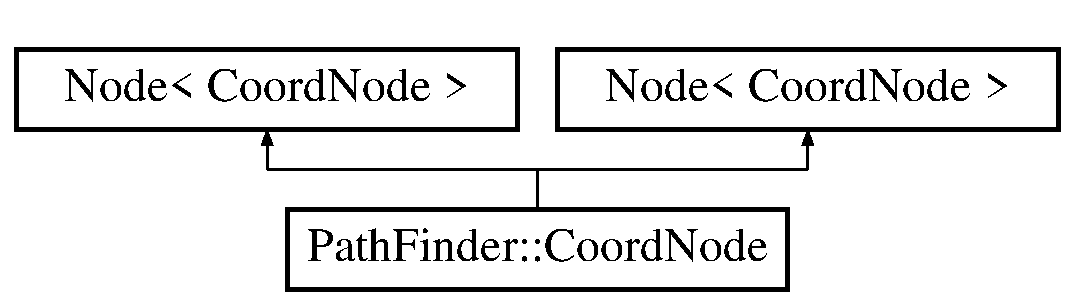
\includegraphics[height=2.000000cm]{class_path_finder_1_1_coord_node}
\end{center}
\end{figure}
\subsection*{Public Member Functions}
\begin{DoxyCompactItemize}
\item 
{\bfseries Coord\+Node} (\hyperlink{class_path_finder}{Path\+Finder} \&path\+Finder, Coordinate coord, Coordinate \&start\+Coord, Length g=Length\+::\+M\+E\+T\+ER $\ast$std\+::numeric\+\_\+limits$<$ double $>$\+::infinity(), std\+::weak\+\_\+ptr$<$ \hyperlink{class_path_finder_1_1_coord_node}{Coord\+Node} $>$ parent=\{\})\hypertarget{class_path_finder_1_1_coord_node_addb07756c6084973916005856b7fb5ff}{}\label{class_path_finder_1_1_coord_node_addb07756c6084973916005856b7fb5ff}

\item 
virtual bool {\bfseries operator==} (const \hyperlink{class_path_finder_1_1_coord_node}{Coord\+Node} \&lhs) const  override\hypertarget{class_path_finder_1_1_coord_node_a9759ffc6e0601d6f7020046bdd999e39}{}\label{class_path_finder_1_1_coord_node_a9759ffc6e0601d6f7020046bdd999e39}

\item 
virtual std\+::vector$<$ \hyperlink{class_path_finder_1_1_coord_node}{Coord\+Node} $>$ {\bfseries get\+\_\+available\+\_\+nodes} (std\+::shared\+\_\+ptr$<$ \hyperlink{class_path_finder_1_1_coord_node}{Coord\+Node} $>$ \&self) override\hypertarget{class_path_finder_1_1_coord_node_a4d454f321e93b41ff8746af411bfc6d6}{}\label{class_path_finder_1_1_coord_node_a4d454f321e93b41ff8746af411bfc6d6}

\item 
{\bfseries Coord\+Node} (\hyperlink{class_path_finder}{Path\+Finder} \&path\+Finder, Coordinate coord, Coordinate \&start\+Coord, Length g=Length\+::\+M\+E\+T\+ER $\ast$std\+::numeric\+\_\+limits$<$ double $>$\+::infinity(), std\+::weak\+\_\+ptr$<$ \hyperlink{class_path_finder_1_1_coord_node}{Coord\+Node} $>$ parent=\{\})\hypertarget{class_path_finder_1_1_coord_node_addb07756c6084973916005856b7fb5ff}{}\label{class_path_finder_1_1_coord_node_addb07756c6084973916005856b7fb5ff}

\item 
virtual bool {\bfseries operator==} (const \hyperlink{class_path_finder_1_1_coord_node}{Coord\+Node} \&lhs) const  override\hypertarget{class_path_finder_1_1_coord_node_a4c72c79b89ada34c9203632add9adbcb}{}\label{class_path_finder_1_1_coord_node_a4c72c79b89ada34c9203632add9adbcb}

\item 
virtual std\+::vector$<$ \hyperlink{class_path_finder_1_1_coord_node}{Coord\+Node} $>$ {\bfseries get\+\_\+available\+\_\+nodes} (std\+::shared\+\_\+ptr$<$ \hyperlink{class_path_finder_1_1_coord_node}{Coord\+Node} $>$ \&self) override\hypertarget{class_path_finder_1_1_coord_node_a4d454f321e93b41ff8746af411bfc6d6}{}\label{class_path_finder_1_1_coord_node_a4d454f321e93b41ff8746af411bfc6d6}

\end{DoxyCompactItemize}
\subsection*{Public Attributes}
\begin{DoxyCompactItemize}
\item 
\hyperlink{class_path_finder}{Path\+Finder} \& {\bfseries path\+Finder}\hypertarget{class_path_finder_1_1_coord_node_a0a17d6e85b89c889b652e152c32a8d88}{}\label{class_path_finder_1_1_coord_node_a0a17d6e85b89c889b652e152c32a8d88}

\item 
Coordinate {\bfseries coord}\hypertarget{class_path_finder_1_1_coord_node_a26f764d5cf615489615f0d255690d1c7}{}\label{class_path_finder_1_1_coord_node_a26f764d5cf615489615f0d255690d1c7}

\item 
Coordinate \& {\bfseries start\+Node\+Coord}\hypertarget{class_path_finder_1_1_coord_node_a8f2b5ba4b954e7c982d82ea9a83901f1}{}\label{class_path_finder_1_1_coord_node_a8f2b5ba4b954e7c982d82ea9a83901f1}

\end{DoxyCompactItemize}
\subsection*{Friends}
\begin{DoxyCompactItemize}
\item 
std\+::ostream \& {\bfseries operator$<$$<$} (std\+::ostream \&lhs, const \hyperlink{class_path_finder_1_1_coord_node}{Coord\+Node} \&rhs)\hypertarget{class_path_finder_1_1_coord_node_a916d53bc1effb05ba13b22a87cd5bf3d}{}\label{class_path_finder_1_1_coord_node_a916d53bc1effb05ba13b22a87cd5bf3d}

\item 
std\+::ostream \& {\bfseries operator$<$$<$} (std\+::ostream \&lhs, const \hyperlink{class_path_finder_1_1_coord_node}{Coord\+Node} \&rhs)\hypertarget{class_path_finder_1_1_coord_node_a916d53bc1effb05ba13b22a87cd5bf3d}{}\label{class_path_finder_1_1_coord_node_a916d53bc1effb05ba13b22a87cd5bf3d}

\end{DoxyCompactItemize}


\subsection{Detailed Description}
implementation of the astar node from \hyperlink{_astar_8hpp_source}{Astar.\+hpp} 

The documentation for this class was generated from the following files\+:\begin{DoxyCompactItemize}
\item 
source/include/Path\+Finder.\+hpp\item 
source/src/main.\+cpp\item 
source/src/Path\+Finder.\+cpp\end{DoxyCompactItemize}

\hypertarget{structstd_1_1hash_3_01_coordinate_01_4}{}\section{std\+:\+:hash$<$ Coordinate $>$ Struct Template Reference}
\label{structstd_1_1hash_3_01_coordinate_01_4}\index{std\+::hash$<$ Coordinate $>$@{std\+::hash$<$ Coordinate $>$}}
\subsection*{Public Member Functions}
\begin{DoxyCompactItemize}
\item 
std\+::size\+\_\+t {\bfseries operator()} (const Coordinate \&coord) const \hypertarget{structstd_1_1hash_3_01_coordinate_01_4_a73c800d2fbb37623684b01a7a6732cd1}{}\label{structstd_1_1hash_3_01_coordinate_01_4_a73c800d2fbb37623684b01a7a6732cd1}

\item 
std\+::size\+\_\+t {\bfseries operator()} (const Coordinate \&coord) const \hypertarget{structstd_1_1hash_3_01_coordinate_01_4_a73c800d2fbb37623684b01a7a6732cd1}{}\label{structstd_1_1hash_3_01_coordinate_01_4_a73c800d2fbb37623684b01a7a6732cd1}

\end{DoxyCompactItemize}


The documentation for this struct was generated from the following files\+:\begin{DoxyCompactItemize}
\item 
source/include/Path\+Finder.\+hpp\item 
source/src/main.\+cpp\end{DoxyCompactItemize}

\hypertarget{structstd_1_1hash_3_01_int_coord_01_4}{}\section{std\+:\+:hash$<$ Int\+Coord $>$ Struct Template Reference}
\label{structstd_1_1hash_3_01_int_coord_01_4}\index{std\+::hash$<$ Int\+Coord $>$@{std\+::hash$<$ Int\+Coord $>$}}
\subsection*{Public Member Functions}
\begin{DoxyCompactItemize}
\item 
std\+::size\+\_\+t {\bfseries operator()} (const \hyperlink{struct_int_coord}{Int\+Coord} \&coord) const \hypertarget{structstd_1_1hash_3_01_int_coord_01_4_ab4ef7f36d5234c766c9a335679656d61}{}\label{structstd_1_1hash_3_01_int_coord_01_4_ab4ef7f36d5234c766c9a335679656d61}

\end{DoxyCompactItemize}


The documentation for this struct was generated from the following file\+:\begin{DoxyCompactItemize}
\item 
source/src/main.\+cpp\end{DoxyCompactItemize}

\hypertarget{structstd_1_1hash_3_01_path_finder_1_1_coord_node_01_4}{}\section{std\+:\+:hash$<$ Path\+Finder\+:\+:Coord\+Node $>$ Struct Template Reference}
\label{structstd_1_1hash_3_01_path_finder_1_1_coord_node_01_4}\index{std\+::hash$<$ Path\+Finder\+::\+Coord\+Node $>$@{std\+::hash$<$ Path\+Finder\+::\+Coord\+Node $>$}}


{\ttfamily \#include $<$Path\+Finder.\+hpp$>$}

\subsection*{Public Member Functions}
\begin{DoxyCompactItemize}
\item 
std\+::size\+\_\+t {\bfseries operator()} (const \hyperlink{class_path_finder_1_1_coord_node}{Path\+Finder\+::\+Coord\+Node} \&node) const \hypertarget{structstd_1_1hash_3_01_path_finder_1_1_coord_node_01_4_ac4d8fe0f857941c8609d92fb08cdcb22}{}\label{structstd_1_1hash_3_01_path_finder_1_1_coord_node_01_4_ac4d8fe0f857941c8609d92fb08cdcb22}

\item 
std\+::size\+\_\+t {\bfseries operator()} (const \hyperlink{class_path_finder_1_1_coord_node}{Path\+Finder\+::\+Coord\+Node} \&node) const \hypertarget{structstd_1_1hash_3_01_path_finder_1_1_coord_node_01_4_ac4d8fe0f857941c8609d92fb08cdcb22}{}\label{structstd_1_1hash_3_01_path_finder_1_1_coord_node_01_4_ac4d8fe0f857941c8609d92fb08cdcb22}

\end{DoxyCompactItemize}


\subsection{Detailed Description}
\subsubsection*{template$<$$>$\\*
struct std\+::hash$<$ Path\+Finder\+::\+Coord\+Node $>$}

hash for the coordinate node class, used for set insertion 

The documentation for this struct was generated from the following files\+:\begin{DoxyCompactItemize}
\item 
source/include/Path\+Finder.\+hpp\item 
source/src/main.\+cpp\end{DoxyCompactItemize}

\hypertarget{struct_int_coord}{}\section{Int\+Coord Struct Reference}
\label{struct_int_coord}\index{Int\+Coord@{Int\+Coord}}
\subsection*{Public Member Functions}
\begin{DoxyCompactItemize}
\item 
{\bfseries Int\+Coord} (int x, int y)\hypertarget{struct_int_coord_a0e71a2a3e23baf93f62aeac59a5e324f}{}\label{struct_int_coord_a0e71a2a3e23baf93f62aeac59a5e324f}

\item 
bool {\bfseries operator==} (const \hyperlink{struct_int_coord}{Int\+Coord} \&lhs) const \hypertarget{struct_int_coord_a366d06d5a1524c48f2a0c374949c9175}{}\label{struct_int_coord_a366d06d5a1524c48f2a0c374949c9175}

\end{DoxyCompactItemize}
\subsection*{Public Attributes}
\begin{DoxyCompactItemize}
\item 
int {\bfseries x}\hypertarget{struct_int_coord_a9d26d75a4264aabef38c15ae27b80ef8}{}\label{struct_int_coord_a9d26d75a4264aabef38c15ae27b80ef8}

\item 
int {\bfseries y}\hypertarget{struct_int_coord_a9491cbad80ce5807fb3e32cfc0bafe79}{}\label{struct_int_coord_a9491cbad80ce5807fb3e32cfc0bafe79}

\end{DoxyCompactItemize}


The documentation for this struct was generated from the following file\+:\begin{DoxyCompactItemize}
\item 
source/src/main.\+cpp\end{DoxyCompactItemize}

\hypertarget{class_map}{}\section{Map Class Reference}
\label{class_map}\index{Map@{Map}}


Dummy \hyperlink{class_map}{Map}.  




{\ttfamily \#include $<$Dummy.\+hpp$>$}

\subsection*{Public Member Functions}
\begin{DoxyCompactItemize}
\item 
\hyperlink{class_map_a2205f271830dc5189f73b7f46da0770e}{Map} (int x=100, int y=100, float obstacles=0.\+25f)
\begin{DoxyCompactList}\small\item\em Constructor. \end{DoxyCompactList}\item 
\hyperlink{class_map_af7916d9ab517490a4a716152569d70ca}{Map} (std\+::vector$<$ std\+::vector$<$ int $>$ $>$ \hyperlink{class_map_a7fbb34f989fcf03bb5717073f882080a}{map})
\begin{DoxyCompactList}\small\item\em Constructor. \end{DoxyCompactList}\item 
void \hyperlink{class_map_a3501397c3e89bf2d874db4541d5bf6e5}{print\+\_\+map} ()
\begin{DoxyCompactList}\small\item\em Print the map. \end{DoxyCompactList}\item 
bool \hyperlink{class_map_a3ad778f596300c295a1ced8f208f3213}{has\+\_\+obstacle} (Coordinate coord, Translation size)
\begin{DoxyCompactList}\small\item\em Returns if position on the map has a obstacle within the robot size. \end{DoxyCompactList}\item 
bool \hyperlink{class_map_a2d929dbb994e4f7d15b392e5b5779cf2}{has\+\_\+passable} (Coordinate coord, Translation size)
\begin{DoxyCompactList}\small\item\em Returns if position on the map has a passable erea within the robot size. \end{DoxyCompactList}\end{DoxyCompactItemize}
\subsection*{Public Attributes}
\begin{DoxyCompactItemize}
\item 
std\+::vector$<$ std\+::vector$<$ int $>$ $>$ \hyperlink{class_map_a7fbb34f989fcf03bb5717073f882080a}{map}\hypertarget{class_map_a7fbb34f989fcf03bb5717073f882080a}{}\label{class_map_a7fbb34f989fcf03bb5717073f882080a}

\begin{DoxyCompactList}\small\item\em Implementation of the map, where\+: 0 = clear, 1 = obstacle, 2 = unexplored. \end{DoxyCompactList}\item 
int \hyperlink{class_map_a762221dfae4de0dd4d63b3dec81ddc02}{sizeX}\hypertarget{class_map_a762221dfae4de0dd4d63b3dec81ddc02}{}\label{class_map_a762221dfae4de0dd4d63b3dec81ddc02}

\begin{DoxyCompactList}\small\item\em The sizes of the map. \end{DoxyCompactList}\item 
int {\bfseries sizeY}\hypertarget{class_map_a3445c0afae51a95d7f98dd57361d04cc}{}\label{class_map_a3445c0afae51a95d7f98dd57361d04cc}

\end{DoxyCompactItemize}


\subsection{Detailed Description}
Dummy \hyperlink{class_map}{Map}. 

\hyperlink{class_map}{Map} for testing the pathfinder 

\subsection{Constructor \& Destructor Documentation}
\index{Map@{Map}!Map@{Map}}
\index{Map@{Map}!Map@{Map}}
\subsubsection[{\texorpdfstring{Map(int x=100, int y=100, float obstacles=0.\+25f)}{Map(int x=100, int y=100, float obstacles=0.25f)}}]{\setlength{\rightskip}{0pt plus 5cm}Map\+::\+Map (
\begin{DoxyParamCaption}
\item[{int}]{x = {\ttfamily 100}, }
\item[{int}]{y = {\ttfamily 100}, }
\item[{float}]{obstacles = {\ttfamily 0.25f}}
\end{DoxyParamCaption}
)}\hypertarget{class_map_a2205f271830dc5189f73b7f46da0770e}{}\label{class_map_a2205f271830dc5189f73b7f46da0770e}


Constructor. 

/param x The width of the map /param y The height of the map /param obstacles Percentage of obstacles in the map \index{Map@{Map}!Map@{Map}}
\index{Map@{Map}!Map@{Map}}
\subsubsection[{\texorpdfstring{Map(std\+::vector$<$ std\+::vector$<$ int $>$ $>$ map)}{Map(std::vector< std::vector< int > > map)}}]{\setlength{\rightskip}{0pt plus 5cm}Map\+::\+Map (
\begin{DoxyParamCaption}
\item[{std\+::vector$<$ std\+::vector$<$ int $>$ $>$}]{map}
\end{DoxyParamCaption}
)}\hypertarget{class_map_af7916d9ab517490a4a716152569d70ca}{}\label{class_map_af7916d9ab517490a4a716152569d70ca}


Constructor. 

/param map The map 

\subsection{Member Function Documentation}
\index{Map@{Map}!has\+\_\+obstacle@{has\+\_\+obstacle}}
\index{has\+\_\+obstacle@{has\+\_\+obstacle}!Map@{Map}}
\subsubsection[{\texorpdfstring{has\+\_\+obstacle(\+Coordinate coord, Translation size)}{has_obstacle(Coordinate coord, Translation size)}}]{\setlength{\rightskip}{0pt plus 5cm}bool Map\+::has\+\_\+obstacle (
\begin{DoxyParamCaption}
\item[{Coordinate}]{coord, }
\item[{Translation}]{size}
\end{DoxyParamCaption}
)}\hypertarget{class_map_a3ad778f596300c295a1ced8f208f3213}{}\label{class_map_a3ad778f596300c295a1ced8f208f3213}


Returns if position on the map has a obstacle within the robot size. 

/param x The x position on the map /param y The y position on the map /param sizeX The width of the robot /param sizeY The height of the robot /return If there is a obstacle found \index{Map@{Map}!has\+\_\+passable@{has\+\_\+passable}}
\index{has\+\_\+passable@{has\+\_\+passable}!Map@{Map}}
\subsubsection[{\texorpdfstring{has\+\_\+passable(\+Coordinate coord, Translation size)}{has_passable(Coordinate coord, Translation size)}}]{\setlength{\rightskip}{0pt plus 5cm}bool Map\+::has\+\_\+passable (
\begin{DoxyParamCaption}
\item[{Coordinate}]{coord, }
\item[{Translation}]{size}
\end{DoxyParamCaption}
)}\hypertarget{class_map_a2d929dbb994e4f7d15b392e5b5779cf2}{}\label{class_map_a2d929dbb994e4f7d15b392e5b5779cf2}


Returns if position on the map has a passable erea within the robot size. 

/param x The x position on the map /param y The y position on the map /param sizeX The width of the robot /param sizeY The height of the robot /return If there is a passable erea \index{Map@{Map}!print\+\_\+map@{print\+\_\+map}}
\index{print\+\_\+map@{print\+\_\+map}!Map@{Map}}
\subsubsection[{\texorpdfstring{print\+\_\+map()}{print_map()}}]{\setlength{\rightskip}{0pt plus 5cm}void Map\+::print\+\_\+map (
\begin{DoxyParamCaption}
{}
\end{DoxyParamCaption}
)}\hypertarget{class_map_a3501397c3e89bf2d874db4541d5bf6e5}{}\label{class_map_a3501397c3e89bf2d874db4541d5bf6e5}


Print the map. 

/return void 

The documentation for this class was generated from the following files\+:\begin{DoxyCompactItemize}
\item 
source/include/Dummy.\+hpp\item 
source/src/Dummy.\+cpp\end{DoxyCompactItemize}

\hypertarget{class_node}{}\section{Node$<$ T $>$ Class Template Reference}
\label{class_node}\index{Node$<$ T $>$@{Node$<$ T $>$}}


{\ttfamily \#include $<$Astar.\+hpp$>$}

\subsection*{Public Member Functions}
\begin{DoxyCompactItemize}
\item 
\hyperlink{class_node_abb1daa11421a3174e22174bc829f3b96}{Node} (Length g=Length\+::\+M\+E\+T\+ER $\ast$0, Length h=Length\+::\+M\+E\+T\+ER $\ast$0, std\+::weak\+\_\+ptr$<$ T $>$ parent=std\+::weak\+\_\+ptr$<$ T $>$())
\item 
virtual bool \hyperlink{class_node_ab37b3f37bf857e602d19f0c16dee99db}{operator==} (const T \&n) const  =0
\item 
virtual std\+::vector$<$ T $>$ \hyperlink{class_node_a21b3fdcc109b15177bd6cb96d9202b13}{get\+\_\+available\+\_\+nodes} (std\+::shared\+\_\+ptr$<$ T $>$ \&self)=0
\item 
bool \hyperlink{class_node_a72a4ef340b3d732c7eae9ad92a2f0cf2}{operator$>$} (const T \&compare) const 
\end{DoxyCompactItemize}
\subsection*{Public Attributes}
\begin{DoxyCompactItemize}
\item 
const Length {\bfseries g}\hypertarget{class_node_a952609bd42c190ae78ca36c7f8aa022d}{}\label{class_node_a952609bd42c190ae78ca36c7f8aa022d}

\item 
Length {\bfseries h}\hypertarget{class_node_a3e4f962de7f9e113dcbaef80f62d7f1d}{}\label{class_node_a3e4f962de7f9e113dcbaef80f62d7f1d}

\item 
Length {\bfseries f}\hypertarget{class_node_ac989fd6403eed28850d38f65e0566d84}{}\label{class_node_ac989fd6403eed28850d38f65e0566d84}

\item 
const std\+::weak\+\_\+ptr$<$ T $>$ {\bfseries parent}\hypertarget{class_node_a25bfffd0d296e093102d92f9dcc82c4e}{}\label{class_node_a25bfffd0d296e093102d92f9dcc82c4e}

\end{DoxyCompactItemize}


\subsection{Detailed Description}
\subsubsection*{template$<$typename T$>$\\*
class Node$<$ T $>$}

abstract class to be implemented by the a star implementation

represents a single node in the a star algorithm 

\subsection{Constructor \& Destructor Documentation}
\index{Node@{Node}!Node@{Node}}
\index{Node@{Node}!Node@{Node}}
\subsubsection[{\texorpdfstring{Node(\+Length g=\+Length\+::\+M\+E\+T\+E\+R $\ast$0, Length h=\+Length\+::\+M\+E\+T\+E\+R $\ast$0, std\+::weak\+\_\+ptr$<$ T $>$ parent=std\+::weak\+\_\+ptr$<$ T $>$())}{Node(Length g=Length::METER *0, Length h=Length::METER *0, std::weak_ptr< T > parent=std::weak_ptr< T >())}}]{\setlength{\rightskip}{0pt plus 5cm}template$<$typename T$>$ {\bf Node}$<$ T $>$\+::{\bf Node} (
\begin{DoxyParamCaption}
\item[{Length}]{g = {\ttfamily Length\+:\+:METER~$\ast$~0}, }
\item[{Length}]{h = {\ttfamily Length\+:\+:METER~$\ast$~0}, }
\item[{std\+::weak\+\_\+ptr$<$ T $>$}]{parent = {\ttfamily std\+:\+:weak\+\_\+ptr$<$T$>$()}}
\end{DoxyParamCaption}
)\hspace{0.3cm}{\ttfamily [inline]}}\hypertarget{class_node_abb1daa11421a3174e22174bc829f3b96}{}\label{class_node_abb1daa11421a3174e22174bc829f3b96}
creates a new node with predefined values as the variables 

\subsection{Member Function Documentation}
\index{Node@{Node}!get\+\_\+available\+\_\+nodes@{get\+\_\+available\+\_\+nodes}}
\index{get\+\_\+available\+\_\+nodes@{get\+\_\+available\+\_\+nodes}!Node@{Node}}
\subsubsection[{\texorpdfstring{get\+\_\+available\+\_\+nodes(std\+::shared\+\_\+ptr$<$ T $>$ \&self)=0}{get_available_nodes(std::shared_ptr< T > &self)=0}}]{\setlength{\rightskip}{0pt plus 5cm}template$<$typename T$>$ virtual std\+::vector$<$T$>$ {\bf Node}$<$ T $>$\+::get\+\_\+available\+\_\+nodes (
\begin{DoxyParamCaption}
\item[{std\+::shared\+\_\+ptr$<$ T $>$ \&}]{self}
\end{DoxyParamCaption}
)\hspace{0.3cm}{\ttfamily [pure virtual]}}\hypertarget{class_node_a21b3fdcc109b15177bd6cb96d9202b13}{}\label{class_node_a21b3fdcc109b15177bd6cb96d9202b13}
get the list of nodes that can be reached from this node

/param self this \index{Node@{Node}!operator==@{operator==}}
\index{operator==@{operator==}!Node@{Node}}
\subsubsection[{\texorpdfstring{operator==(const T \&n) const  =0}{operator==(const T &n) const  =0}}]{\setlength{\rightskip}{0pt plus 5cm}template$<$typename T$>$ virtual bool {\bf Node}$<$ T $>$\+::operator== (
\begin{DoxyParamCaption}
\item[{const T \&}]{n}
\end{DoxyParamCaption}
) const\hspace{0.3cm}{\ttfamily [pure virtual]}}\hypertarget{class_node_ab37b3f37bf857e602d19f0c16dee99db}{}\label{class_node_ab37b3f37bf857e602d19f0c16dee99db}
checks if two nodes can be considered equal for the algorithm

/return true if the two nodes are approximately equal \index{Node@{Node}!operator$>$@{operator$>$}}
\index{operator$>$@{operator$>$}!Node@{Node}}
\subsubsection[{\texorpdfstring{operator$>$(const T \&compare) const }{operator>(const T &compare) const }}]{\setlength{\rightskip}{0pt plus 5cm}template$<$typename T$>$ bool {\bf Node}$<$ T $>$\+::operator$>$ (
\begin{DoxyParamCaption}
\item[{const T \&}]{compare}
\end{DoxyParamCaption}
) const\hspace{0.3cm}{\ttfamily [inline]}}\hypertarget{class_node_a72a4ef340b3d732c7eae9ad92a2f0cf2}{}\label{class_node_a72a4ef340b3d732c7eae9ad92a2f0cf2}
compares two nodes for checking which should be evaluated first 

The documentation for this class was generated from the following file\+:\begin{DoxyCompactItemize}
\item 
source/include/Astar.\+hpp\end{DoxyCompactItemize}

\hypertarget{class_path_finder}{}\section{Path\+Finder Class Reference}
\label{class_path_finder}\index{Path\+Finder@{Path\+Finder}}


{\ttfamily \#include $<$Path\+Finder.\+hpp$>$}

\subsection*{Classes}
\begin{DoxyCompactItemize}
\item 
class \hyperlink{class_path_finder_1_1_coord_node}{Coord\+Node}
\end{DoxyCompactItemize}
\subsection*{Public Member Functions}
\begin{DoxyCompactItemize}
\item 
\hyperlink{class_path_finder_a820a04a9ec65349b10cf21898bc89227}{Path\+Finder} (\hyperlink{class_map}{Map} \&map, Translation robot\+Box)
\item 
virtual bool \hyperlink{class_path_finder_acada549f3bc9792d9c4031484f017725}{get\+\_\+path\+\_\+to\+\_\+coordinate} (Coordinate start, Coordinate goal, std\+::vector$<$ Coordinate $>$ \&path)
\item 
\hyperlink{class_path_finder_a820a04a9ec65349b10cf21898bc89227}{Path\+Finder} (\hyperlink{class_map}{Map} \&map, Translation robot\+Box)
\item 
virtual bool \hyperlink{class_path_finder_a0c572b99f2c8cb944ebf49ad502cba7f}{get\+\_\+path\+\_\+to\+\_\+coordinate} (Coordinate start, Coordinate goal, std\+::vector$<$ Coordinate $>$ \&path)
\end{DoxyCompactItemize}


\subsection{Detailed Description}
interface for a pathfinder module

computes a path between two points on a map 

\subsection{Constructor \& Destructor Documentation}
\index{Path\+Finder@{Path\+Finder}!Path\+Finder@{Path\+Finder}}
\index{Path\+Finder@{Path\+Finder}!Path\+Finder@{Path\+Finder}}
\subsubsection[{\texorpdfstring{Path\+Finder(\+Map \&map, Translation robot\+Box)}{PathFinder(Map &map, Translation robotBox)}}]{\setlength{\rightskip}{0pt plus 5cm}Path\+Finder\+::\+Path\+Finder (
\begin{DoxyParamCaption}
\item[{{\bf Map} \&}]{map, }
\item[{Translation}]{robot\+Box}
\end{DoxyParamCaption}
)}\hypertarget{class_path_finder_a820a04a9ec65349b10cf21898bc89227}{}\label{class_path_finder_a820a04a9ec65349b10cf21898bc89227}
Constructor

/param map Reference to the world map /param robot\+Size Reference to the robot size \index{Path\+Finder@{Path\+Finder}!Path\+Finder@{Path\+Finder}}
\index{Path\+Finder@{Path\+Finder}!Path\+Finder@{Path\+Finder}}
\subsubsection[{\texorpdfstring{Path\+Finder(\+Map \&map, Translation robot\+Box)}{PathFinder(Map &map, Translation robotBox)}}]{\setlength{\rightskip}{0pt plus 5cm}Path\+Finder\+::\+Path\+Finder (
\begin{DoxyParamCaption}
\item[{{\bf Map} \&}]{map, }
\item[{Translation}]{robot\+Box}
\end{DoxyParamCaption}
)}\hypertarget{class_path_finder_a820a04a9ec65349b10cf21898bc89227}{}\label{class_path_finder_a820a04a9ec65349b10cf21898bc89227}
Constructor

/param map Reference to the world map /param robot\+Size Reference to the robot size 

\subsection{Member Function Documentation}
\index{Path\+Finder@{Path\+Finder}!get\+\_\+path\+\_\+to\+\_\+coordinate@{get\+\_\+path\+\_\+to\+\_\+coordinate}}
\index{get\+\_\+path\+\_\+to\+\_\+coordinate@{get\+\_\+path\+\_\+to\+\_\+coordinate}!Path\+Finder@{Path\+Finder}}
\subsubsection[{\texorpdfstring{get\+\_\+path\+\_\+to\+\_\+coordinate(\+Coordinate start, Coordinate goal, std\+::vector$<$ Coordinate $>$ \&path)}{get_path_to_coordinate(Coordinate start, Coordinate goal, std::vector< Coordinate > &path)}}]{\setlength{\rightskip}{0pt plus 5cm}bool Path\+Finder\+::get\+\_\+path\+\_\+to\+\_\+coordinate (
\begin{DoxyParamCaption}
\item[{Coordinate}]{start, }
\item[{Coordinate}]{goal, }
\item[{std\+::vector$<$ Coordinate $>$ \&}]{path}
\end{DoxyParamCaption}
)\hspace{0.3cm}{\ttfamily [virtual]}}\hypertarget{class_path_finder_acada549f3bc9792d9c4031484f017725}{}\label{class_path_finder_acada549f3bc9792d9c4031484f017725}
Returns a path between two points

This function computes a path from start to goal, based on the map and robot size given in the constructor

/param start The start coordinate /param goal The goal coordinate /param path Vector where the path need to be written to /return If it was able to find a path \index{Path\+Finder@{Path\+Finder}!get\+\_\+path\+\_\+to\+\_\+coordinate@{get\+\_\+path\+\_\+to\+\_\+coordinate}}
\index{get\+\_\+path\+\_\+to\+\_\+coordinate@{get\+\_\+path\+\_\+to\+\_\+coordinate}!Path\+Finder@{Path\+Finder}}
\subsubsection[{\texorpdfstring{get\+\_\+path\+\_\+to\+\_\+coordinate(\+Coordinate start, Coordinate goal, std\+::vector$<$ Coordinate $>$ \&path)}{get_path_to_coordinate(Coordinate start, Coordinate goal, std::vector< Coordinate > &path)}}]{\setlength{\rightskip}{0pt plus 5cm}virtual bool Path\+Finder\+::get\+\_\+path\+\_\+to\+\_\+coordinate (
\begin{DoxyParamCaption}
\item[{Coordinate}]{start, }
\item[{Coordinate}]{goal, }
\item[{std\+::vector$<$ Coordinate $>$ \&}]{path}
\end{DoxyParamCaption}
)\hspace{0.3cm}{\ttfamily [virtual]}}\hypertarget{class_path_finder_a0c572b99f2c8cb944ebf49ad502cba7f}{}\label{class_path_finder_a0c572b99f2c8cb944ebf49ad502cba7f}
Returns a path between two points

This function computes a path from start to goal, based on the map and robot size given in the constructor

/param start The start coordinate /param goal The goal coordinate /param path Vector where the path need to be written to /return If it was able to find a path 

The documentation for this class was generated from the following files\+:\begin{DoxyCompactItemize}
\item 
source/include/Path\+Finder.\+hpp\item 
source/src/main.\+cpp\item 
source/src/Path\+Finder.\+cpp\end{DoxyCompactItemize}

%--- End generated contents ---

% Index
\backmatter
\newpage
\phantomsection
\clearemptydoublepage
\addcontentsline{toc}{chapter}{Index}
\printindex

\end{document}
